\chapter{Parte II — Sistema de localización basado en consentimiento}\label{cap:parte2}

\section{Enfoque}
La guía pide un sistema que localice un teléfono a partir de su número, con aplicación cliente, backend, base de datos, mapa e historial, y advierte que el ejercicio es académico y que no se puede rastrear a nadie sin su autorización. Un localizador es, por naturaleza, una herramienta que puede usarse para acechar a una persona. Por eso el diseño parte de una regla: \textbf{nadie ve la ubicación de nadie sin un permiso expreso, temporal, revocable y visible para el titular}. El código está en la carpeta \cod{parte2/} del repositorio.

Se eligió una aplicación web progresiva (PWA) en lugar de una app nativa: el navegador del teléfono ofrece la API de geolocalización con su propio aviso de permiso, no requiere publicar en una tienda y se puede probar de punta a punta en el laboratorio.

\section{Arquitectura}
\begin{figure}[H]\centering
\begin{tikzpicture}[font=\small,
  box/.style={draw,rounded corners,align=center,minimum height=1.1cm,fill=#1},
  box/.default=white, >=Stealth]
\node[box=bgreal!10,minimum width=3.4cm] (dev) {\textbf{Titular}\\PWA en el teléfono\\GPS del navegador};
\node[box=bgsint!10,minimum width=3.4cm,below=1.6cm of dev] (view) {\textbf{Observador}\\Panel web\\Mapa Leaflet};
\node[box=udazul!10,minimum width=4.6cm,minimum height=3.9cm,anchor=west] (api) at ($(dev.east)!0.5!(view.east)+(3.3,0)$) {\textbf{API REST (FastAPI)}\\[4pt]\scriptsize Autenticación por código\\\scriptsize Sesiones con token\\\scriptsize Permisos y vencimiento\\\scriptsize Ubicaciones e historial\\\scriptsize Geocercas y alertas\\\scriptsize Registro de actividad\\\scriptsize Cabeceras de seguridad};
\node[box=black!5,minimum width=2.8cm,right=1.4cm of api,yshift=0.9cm] (db) {\textbf{Base de datos}\\SQLite\\(SQLAlchemy)};
\node[box=black!5,minimum width=2.8cm,right=1.4cm of api,yshift=-0.9cm] (sms) {\textbf{SMS}\\simulado\\(consola)};
\node[box=black!5,minimum width=3.4cm,below=0.9cm of view] (osm) {Teselas OpenStreetMap\\(requieren Internet)};
\draw[->] (dev.east) -- node[above,sloped,font=\scriptsize]{POST /locations} (api.west|-dev.east);
\draw[<->] (view.east) -- node[below,sloped,font=\scriptsize]{GET /grants/\{id\}/…} (api.west|-view.east);
\draw[<->] (api.east|-db) -- (db.west);
\draw[->] (api.east|-sms) -- (sms.west);
\draw[->,dashed] (view.south) -- (osm.north);
\end{tikzpicture}
\caption{Arquitectura de la Parte II. La API es el único punto que decide quién ve qué; el navegador del observador nunca recibe ubicaciones sin un permiso vigente.}\end{figure}

\begin{table}[H]\centering\small\caption{Componentes de la Parte II.}
\begin{tabularx}{\linewidth}{@{}p{3cm}X@{}}\toprule
\textbf{Componente} & \textbf{Implementación}\\\midrule
Backend & Python 3.13, FastAPI 0.165, SQLAlchemy 2.1.9; fábrica \cod{create\_app(settings)} configurable por variables \cod{LOC\_*}\\
Base de datos & SQLite por defecto con claves foráneas activas; cualquier URL de SQLAlchemy (por ejemplo PostgreSQL) es posible pero no se probó\\
Cliente & HTML, CSS y JavaScript sin frameworks; Leaflet 1.9.4 incluido en el repositorio (sin CDN); manifiesto PWA\\
Modelo de datos & \cod{users}, \cod{phone\_codes}, \cod{devices}, \cod{sessions}, \cod{grants}, \cod{locations}, \cod{geofences}, \cod{geofence\_states}, \cod{alerts}, \cod{audit\_log}\\
Geocodificación & Cliente de Nominatim con caché, 1 consulta/s y coordenadas redondeadas a 4 decimales; desactivado por defecto\\
Mantenimiento & \cod{python -m app.maintenance} purga ubicaciones más antiguas que la retención (30 días por defecto)\\
\bottomrule\end{tabularx}\end{table}

\subsection{API}
\begin{table}[H]\centering\small\caption{Endpoints de la API REST.}
\begin{tabularx}{\linewidth}{@{}p{1.6cm}p{5.6cm}X@{}}\toprule
\textbf{Perfil} & \textbf{Endpoint} & \textbf{Función}\\\midrule
Ambos & \cod{POST /api/auth/request-code} & Envía código de 6 dígitos al número (E.164)\\
 & \cod{POST /api/auth/verify} & Verifica el código y entrega el token de sesión\\
 & \cod{POST /api/auth/logout}, \cod{GET|DELETE /api/me} & Cierra sesión; consulta o elimina la cuenta\\\midrule
Titular & \cod{GET /api/device/status} & Estado, solicitudes y permisos\\
 & \cod{PUT /api/device/sharing} & Activa o pausa el uso compartido y fija el intervalo\\
 & \cod{POST|DELETE /api/device/locations} & Envía una ubicación; borra todo el historial\\
 & \cod{POST /api/device/grants/\{id\}/}\newline\cod{approve|deny|revoke} & Decide sobre cada observador\\
 & \cod{GET /api/device/audit} & Registro de actividad: quién pidió, aprobó y consultó\\\midrule
Observador & \cod{POST /api/viewer/requests} & Pide permiso con un mensaje\\
 & \cod{GET /api/viewer/grants} & Estado de sus solicitudes\\
 & \cod{GET …/grants/\{id\}/}\newline\cod{latest|history|stats} & Última ubicación, historial y distancia\\
 & \cod{GET|POST|DELETE}\newline\cod{…/grants/\{id\}/geofences} & Zonas (máximo 10 por permiso)\\
 & \cod{GET …/grants/\{id\}/alerts}, \cod{GET /api/viewer/geocode} & Alertas de zona; dirección aproximada\\
\bottomrule\end{tabularx}\end{table}

\section{Flujo de uso}
\begin{enumerate}
\item \textbf{Registro.} La persona escribe su número; recibe un código de 6 dígitos por SMS y obtiene una sesión.
\item \textbf{Estado inicial.} El uso compartido nace apagado y un aviso permanente indica si se está compartiendo.
\item \textbf{Solicitud.} El observador pide permiso con un mensaje que explica quién es y para qué. No ve nada todavía.
\item \textbf{Decisión.} El titular aprueba por 1 a 90 días, con o sin historial, o rechaza (24~h de espera antes de poder pedir otra vez).
\item \textbf{Ubicación.} El titular activa el uso compartido; el navegador pide el permiso de GPS y envía la posición cada 10 minutos (configurable) o a mano.
\item \textbf{Consulta.} El observador autorizado ve el mapa, el recorrido, estadísticas y crea zonas con alertas de entrada y salida.
\item \textbf{Control.} El titular ve cada consulta en su registro, revoca cuando quiera y puede borrar su historial o su cuenta.
\end{enumerate}

\section{Evidencia de funcionamiento}
El script \cod{tests/e2e\_navegador.py} levanta el servidor y recorre el flujo en Google Chrome con dos personas distintas: el titular en una pantalla de teléfono con GPS simulado en Bogotá y el observador en una de escritorio. Las capturas son de esa ejecución. Las teselas de OpenStreetMap necesitan Internet, por eso el mapa aparece sin fondo; los marcadores, el recorrido y las zonas sí se dibujan.

\begin{figure}[H]\centering
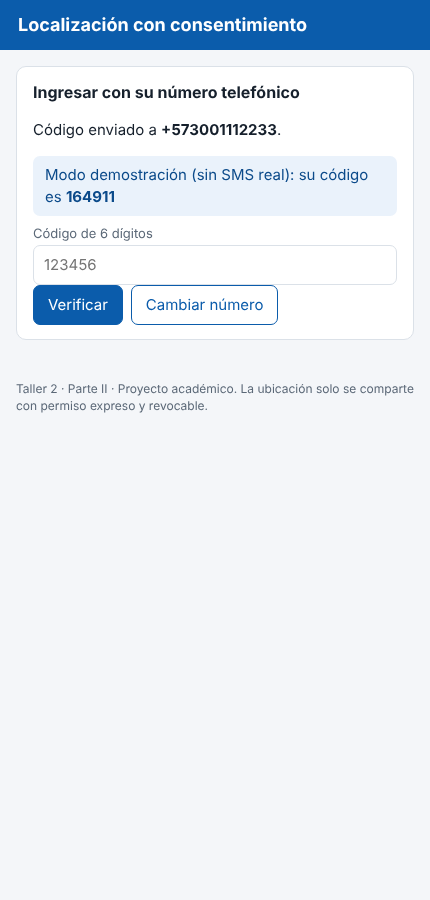
\includegraphics[height=8.6cm]{fig/01-registro-codigo.png}\hspace{0.6cm}
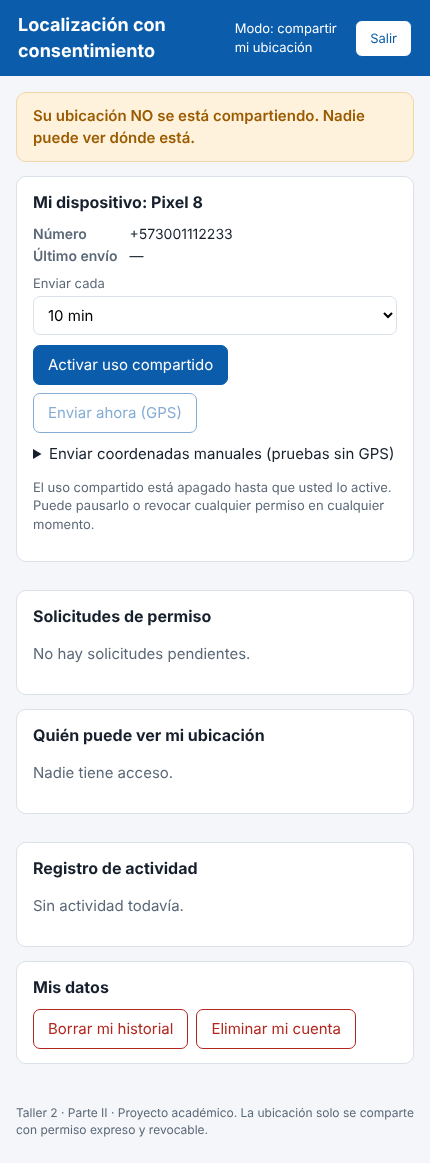
\includegraphics[height=8.6cm]{fig/02-dispositivo-apagado.png}
\caption{Registro por número con código (izquierda; en modo demostración el código se muestra en pantalla porque el SMS es simulado) y estado inicial del titular: la ubicación no se comparte (derecha).}\end{figure}
\fig[0.8]{03-observador-pendiente.png}{El observador pidió permiso: la solicitud queda pendiente y no hay botón de mapa.}
\begin{figure}[H]\centering
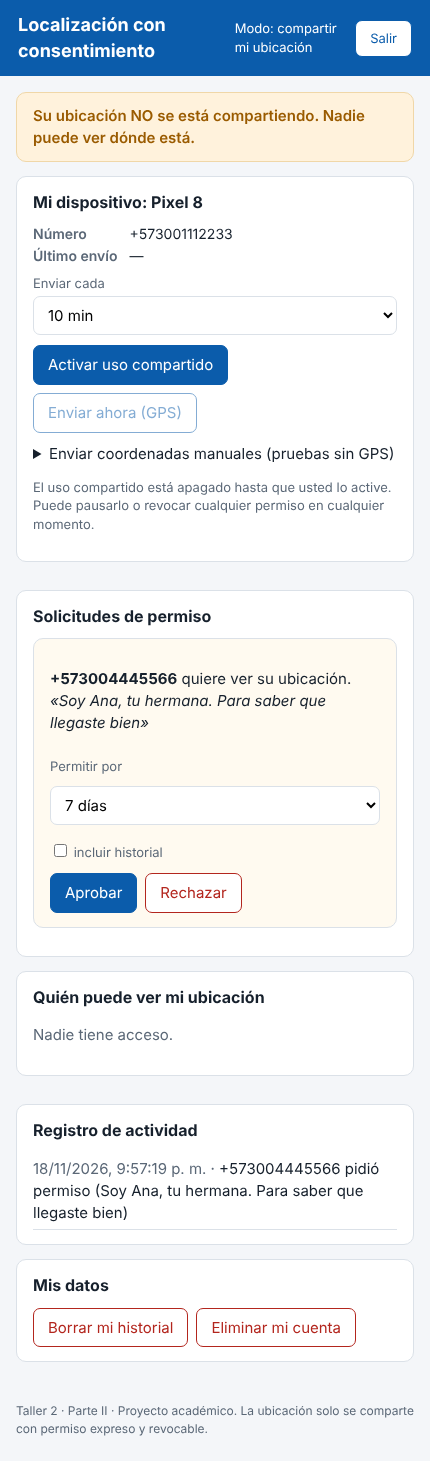
\includegraphics[height=10cm]{fig/04-solicitud-recibida.png}\hspace{0.6cm}
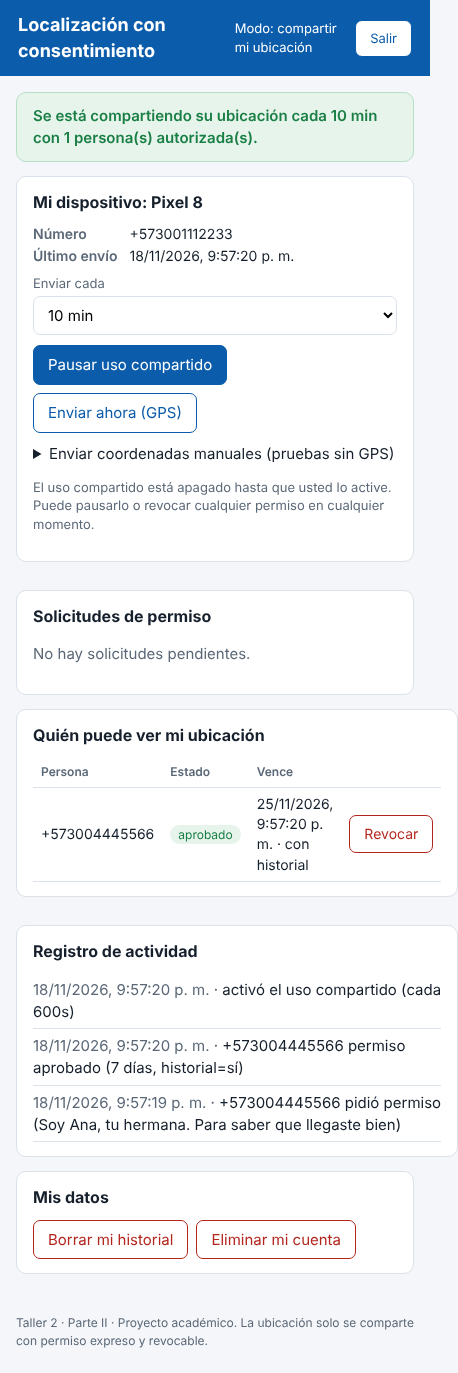
\includegraphics[height=10cm]{fig/05-dispositivo-compartiendo.png}
\caption{El titular recibe la solicitud con el mensaje del observador y elige duración e historial (izquierda). Tras aprobar 7 días con historial y activar el uso compartido, el aviso cambia y el registro de actividad anota cada paso (derecha).}\end{figure}
\fig[0.8]{06-mapa-historial.png}{El observador autorizado ve la última posición, el recorrido y la distancia recorrida.}
\fig[0.8]{07-zona-alerta.png}{Zona ``Casa'' de 300~m y alerta de salida cuando el titular envía una posición a unos 4,6~km.}
\begin{figure}[H]\centering
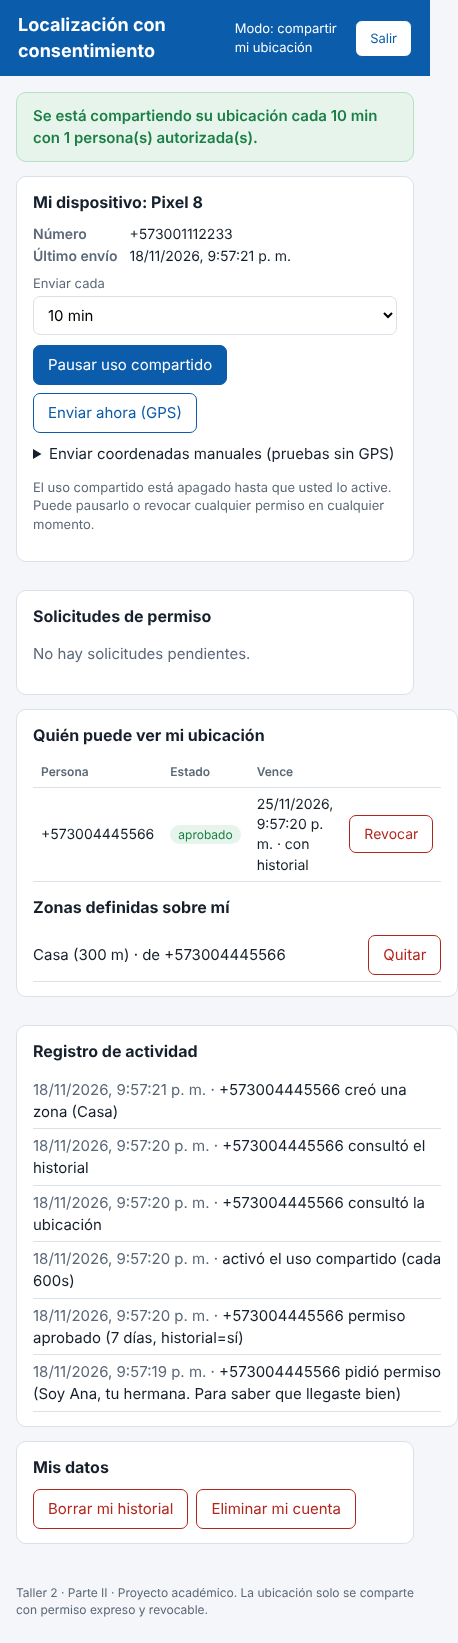
\includegraphics[height=10cm]{fig/08-dueno-registro.png}
\caption{El titular ve quién consultó su ubicación y cuándo, y puede revocar.}\end{figure}
\fig[0.8]{09-acceso-revocado.png}{Tras la revocación, el observador pierde el acceso en la siguiente petición.}

La prueba encontró un fallo real de la interfaz: dos refrescos del mapa en paralelo dibujaban el marcador dos veces. Se corrigió con un contador de secuencia que descarta las respuestas viejas.

\fig[0.98]{term-p2-tests.png}{Las 61 pruebas automáticas de la API: autenticación, consentimiento, ubicaciones, geocercas, retención y borrado.}

\section{Cobertura de requisitos}
\begin{table}[H]\centering\small\caption{Requisitos de la guía y estado.}
\begin{tabularx}{\linewidth}{@{}p{4.6cm}p{1.6cm}X@{}}\toprule
\textbf{Requisito} & \textbf{Estado} & \textbf{Detalle}\\\midrule
Registro por número y verificación por SMS & Parcial & Código de 6 dígitos implementado; envío de SMS simulado (consola), con interfaz para un proveedor real\\
Solicitud y captura de ubicación & Cumplido & GPS del navegador con permiso; envío manual o coordenadas para pruebas\\
Actualización periódica & Cumplido & Intervalo configurable, 10 min por defecto; mientras la página esté abierta\\
Visualización en mapa & Cumplido & Leaflet con OpenStreetMap\\
Historial por fecha y hora & Cumplido & Recorrido y lista con marca de tiempo, si el titular lo permite\\
Alertas por zona (opcional) & Cumplido & Entrada y salida; la primera lectura fija el estado sin alertar\\
Acceso seguro & Cumplido & Token por sesión, permisos por observador\\
API REST y base de datos & Cumplido & FastAPI; SQLite (PostgreSQL, MongoDB y Firebase no se probaron)\\
Geocodificación inversa & Parcial & Implementada, desactivada sin red\\
Estadísticas de movimiento & Cumplido & Puntos y distancia (fórmula de Haversine)\\
Panel web & Cumplido & Interfaz de observador\\
Bot de Telegram (opcional) & No & No implementado\\
Varios dispositivos & No & Un dispositivo por cuenta\\
Ahorro de batería & No & Un navegador no garantiza envíos con la pantalla bloqueada\\
\bottomrule\end{tabularx}\end{table}

\section{Revisión de seguridad del prototipo}
La revisión sigue los controles de autenticación, sesión y validación de OWASP ASVS \cite{owasp} adaptados al riesgo propio de un localizador.
\begin{table}[H]\centering\small\caption{Riesgos y controles implementados.}
\begin{tabularx}{\linewidth}{@{}p{4.2cm}X@{}}\toprule
\textbf{Riesgo} & \textbf{Control}\\\midrule
Seguimiento encubierto & Compartir apagado por defecto; aviso permanente; ver exige aprobación explícita\\
Permiso indefinido & Vence entre 1 y 90 días; el vencimiento se aplica en cada consulta\\
No poder retirar el permiso & Revocación inmediata; el observador pierde acceso en la siguiente petición\\
Consultas ocultas & Registro de actividad visible para el titular\\
Hostigamiento con solicitudes & 5 solicitudes por día por observador; 24~h de espera tras un rechazo\\
Saber si un número usa el sistema & Respuestas idénticas exista o no el número\\
Adivinar el código & 6 dígitos de \cod{secrets}; guardado solo como HMAC-SHA256; 5 intentos; vigencia 10 min; 3 códigos por 10 min por número y 20 por hora por IP\\
Robo de la base de datos & Tokens guardados como SHA-256; nunca en claro\\
XSS & CSP restrictiva; la interfaz no usa \cod{innerHTML}; datos insertados con \cod{textContent}\\
Fuga por caché o referer & \cod{Cache-Control: no-store} en la API; \cod{Referrer-Policy: no-referrer}; \cod{nosniff}\\
Acumulación de datos & Retención de 30 días; borrar historial y eliminar cuenta\\
\bottomrule\end{tabularx}\end{table}

\section{Privacidad y marco legal}
El diseño sigue los principios de la Ley 1581 de 2012: el consentimiento es previo, expreso e informado (el observador explica quién es y para qué, el titular decide); la finalidad y el tiempo están acotados (vencimiento); el acceso está restringido a quien el titular autoriza; y el titular puede conocer (registro de actividad) y suprimir sus datos (borrado). En un despliegue real harían falta además una política de tratamiento publicada, HTTPS obligatorio (la geolocalización del navegador lo exige fuera de \emph{localhost}) y un proveedor de SMS con acuerdo de tratamiento de datos.

\section{Límites}
Es una aplicación web, no nativa; el SMS es simulado; no hay bot de Telegram ni varios dispositivos por cuenta; la base de datos es SQLite; los mosaicos del mapa requieren Internet; y la seguridad se comprobó con pruebas propias, sin auditoría independiente.
